\section{Richard-Germay-Detournay Family of Bit Model}
%\section{RGD Family of Models}
\label{ch:rgdmodels}

\subsection{Introduction}
While the current project focuses on drill string models, it is natural to couple a string model with a bit model. The Richard-Germay-Detournay family of bit models (RGD models) represents theoretical bit-rock interactions. They use a more sophisticated approach than many bit models and are, therefore, of interest. The RGD model is developed by Richard et al., 2007\ \cite{ref:richard2007a}, which simulates coupled axial and torsional vibration mode through bit-rock interaction. The model has been applied to numerous drill-string models to model bit-rock interactions.

\subsection{RGD Model}
The model combines governing equations of motions (axial and torsional) with bit-rock interface law which leads to a state-dependent delay system. In other words, it is a 2 DOF bit model which simulates the torsional and axial modes at bit which are coupled by bit-rock interaction model by depth of cut. Also, the model takes into account the loss of contact at wearflat/rock interface caused by axial vibration of the bit through a discontinuous boundary conditions. A brief description of the mathematical background is shown in \figurename~\ref{figure_RGD_Summary}.  functions $T_c$, $T_f$, $W_C$ and $W_f$ \reviewcomment{Define parameters.}\resolvedcomment{} are defined with respect to the drilling regime which reflects the discontinuous boundary conditions (see \figurename~\ref{figure_RGD_Summary}). \needsclarification{} The drilling regimes are classified as cutting ($\omega>0, d>0$), sticking ($\omega=0, d>0$), sliding ($\omega>0, d=0$) and off-bottom ($\omega>0, d<0$). \reviewcomment{Are these intended to be ordered or numbered?}\resolvedcomment{} 
\begin{figure}
  \centering
  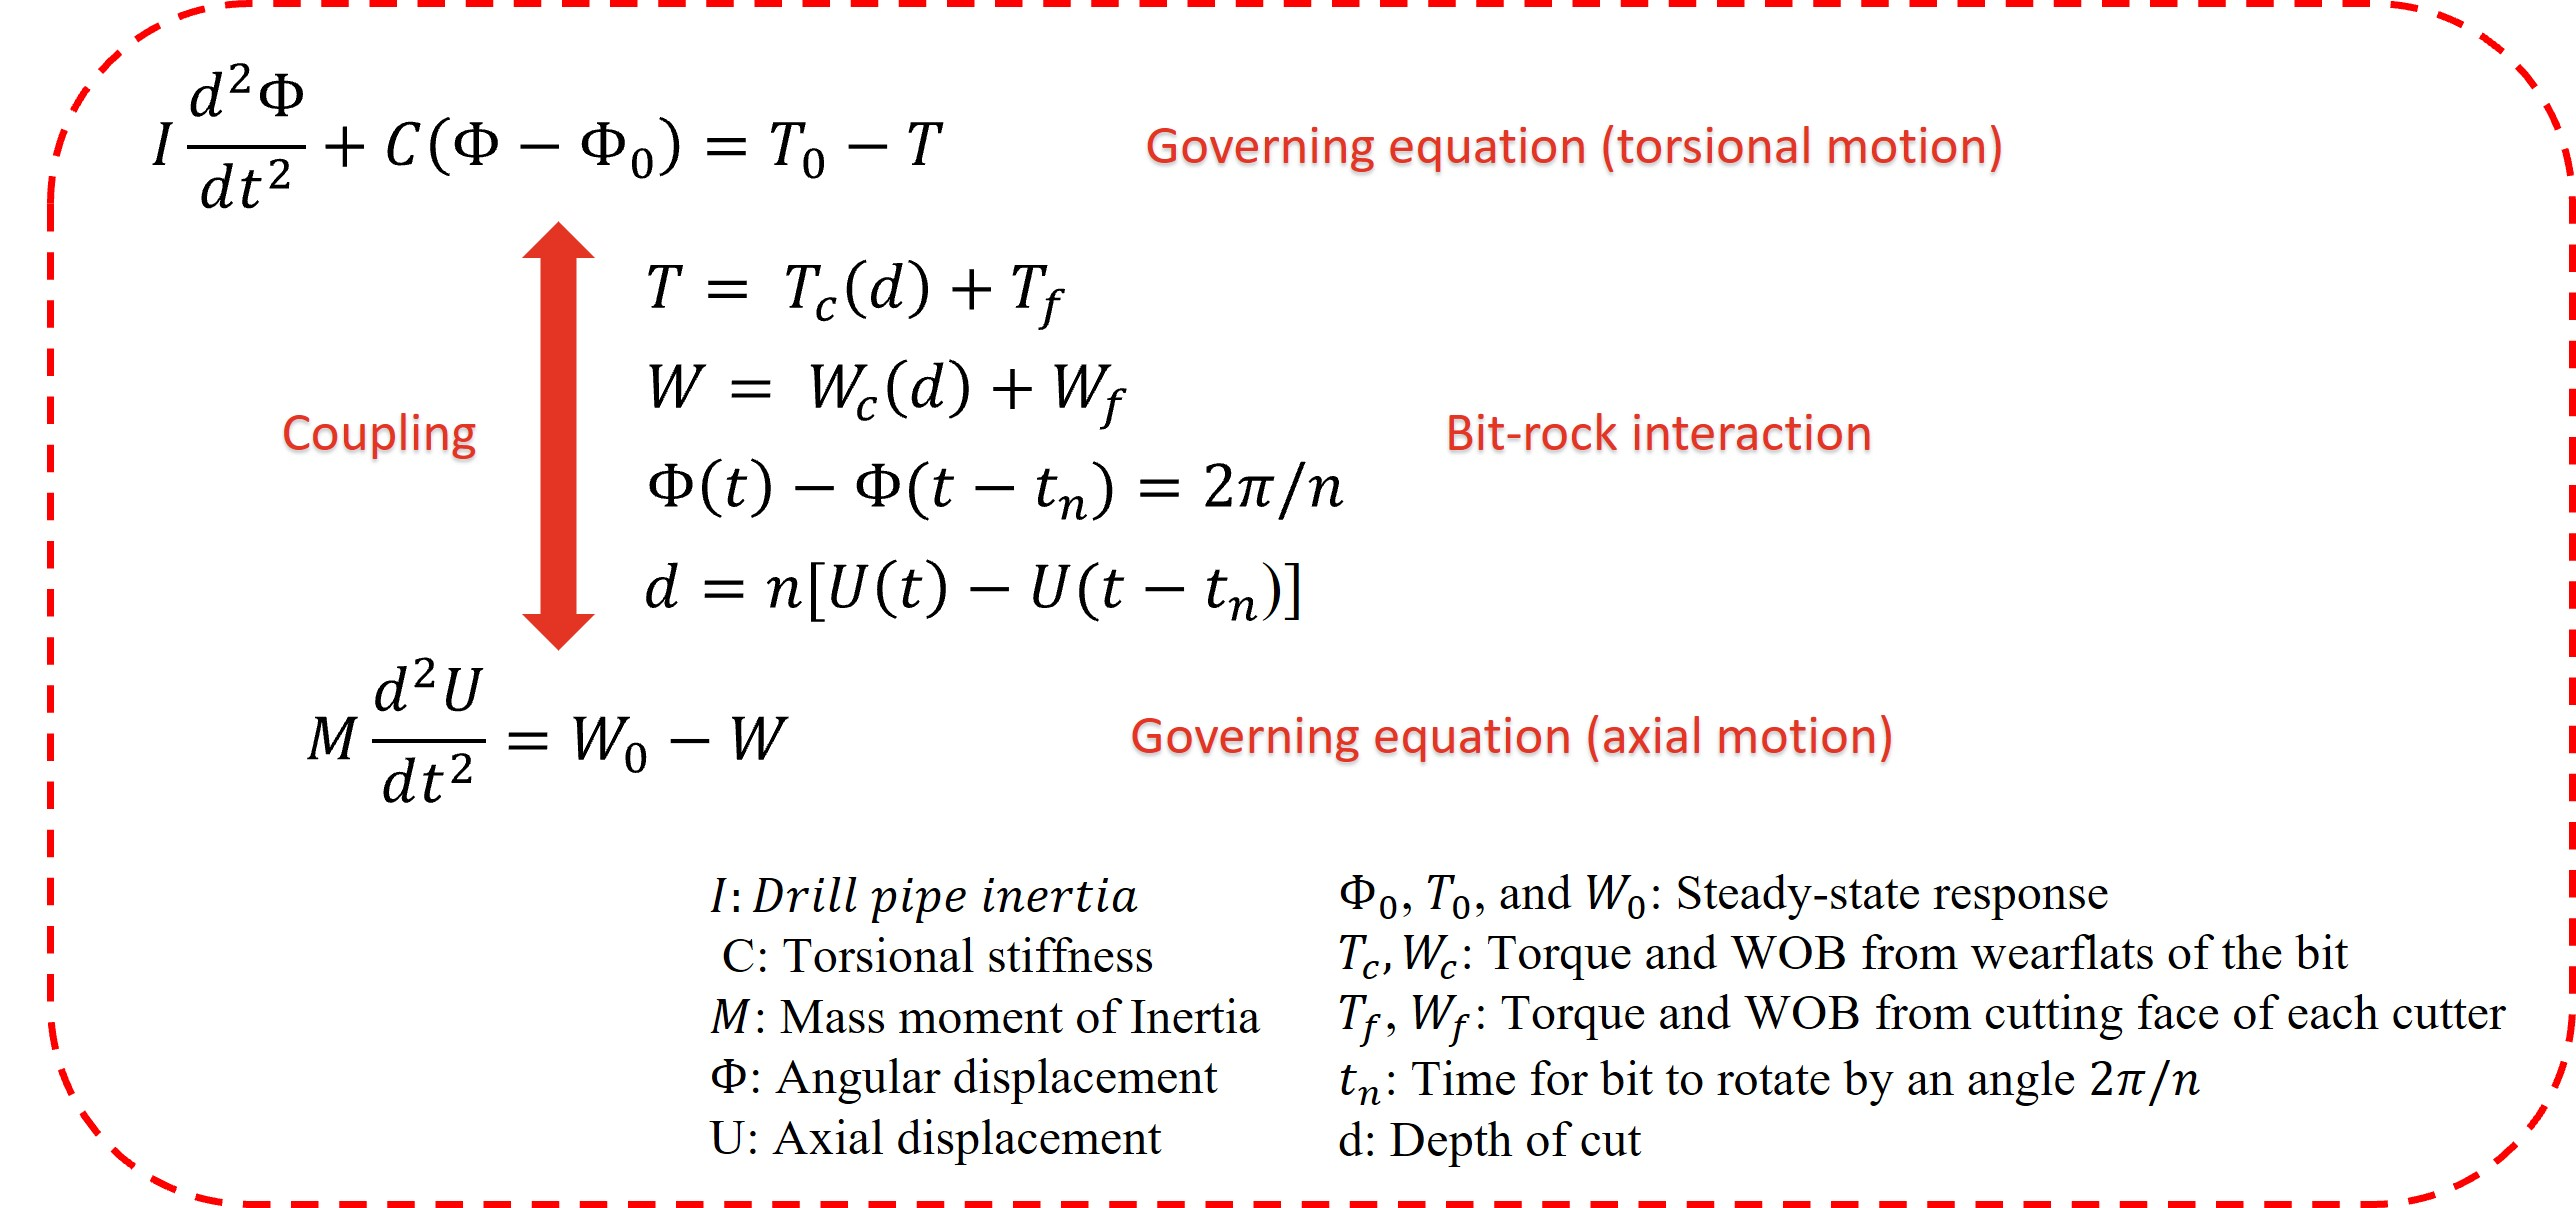
\includegraphics[width=5in]{RGD_summary}
  \caption[Mathematical description of RGD model]{Mathematical description of RGD model.}\label{figure_RGD_Summary}
\end{figure}
The base assumptions of the model are:
\begin{bulletedlist}
	\item Constant angular velocity and upward force at the top of the drill string.
	\item A vertical borehole.
	\item No lateral motion of the bit.
	\item Most of the energy dissipation occurs at the bit-rock interface.
    \item No additional damping parameters other than energy dissipation at the bit-rock interface.
\end{bulletedlist}
Since it is a bit model, not a drill string model, and it is limited to vertical well, this model was not selected for the evaluation. However, the source code of 2 DOF RGD bit model is available and mathematical details based on the code can be seen in \appendixname~\ref{ap:rgbworkflow}. \reviewcomment{Appendix is for spectral method?} \resolvedcomment{}

\subsection{Extended RGD Model}
Numerous drill string models benchmarked RGD model for bit-rock interactions. \figurename~\ref{model_develop_figure} illustrates the development of the RGD model.
\begin{figure}
  \centering
  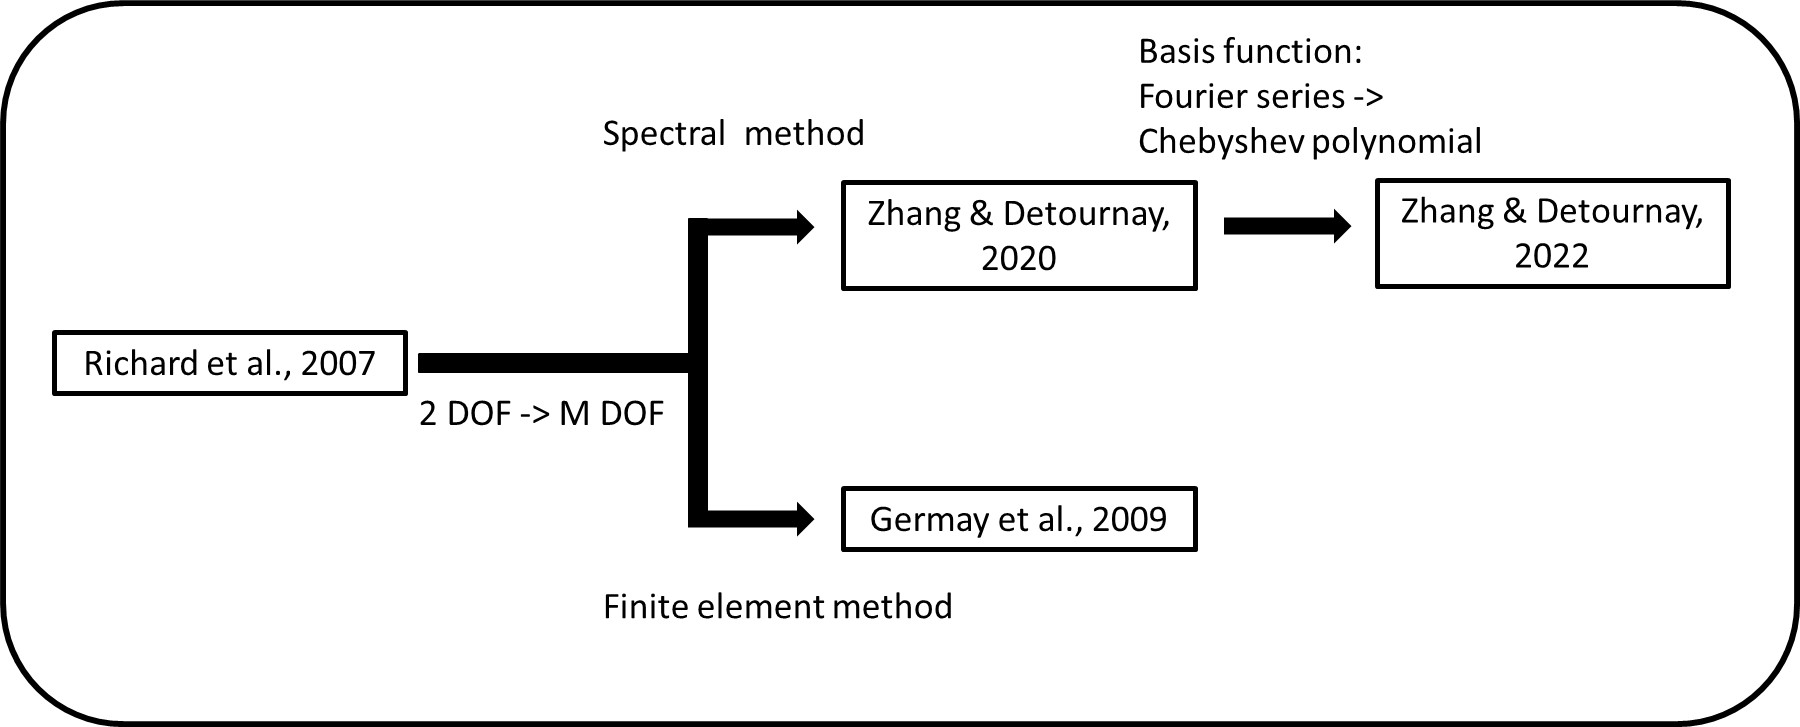
\includegraphics[width=5in]{ModelDevelop}
  \caption[RGD model development]{RGD model development.}\label{model_develop_figure}
\end{figure} 
Germay extended the 2 DOF RGD model to a continumm model by applying FEM approach in \referencename~\cite{ref:germay2009a} \reviewcomment{Now this is becoming a drill string \emph{and} bit model. We need to clarify the wording.} This model was able to simulate the stick \reviewcomment{Full stick?} phase that occurred by vibration higher than the first natural torsional frequency since it captured behaviour of higher frequency from increased degrees of freedom. Similarly, Zhang increased the DOF of the model by discretizing the drill string and implementing the spectral method. This further improved the computational efficiency by applying Chebyshev polynomial as a basis function (see \referencename~\cite{ref:zhang2020a}). The model was able to simulate axial and torsional vibrations, including stick-slip events, with enhanced computation efficiency compared to the FEM approach. The source codes for the models were not provided, therefore, we could not evalutate in this project. \reviewcomment{Source code for one or both?}\resolvedcomment{}. However, these models can be good candidates for further study. 